\chapter{Recommender systems}

In a world of information overload, automatic filtering tools are essential to
extract relevant information from basic noise. In the field of e-commerce,
recommender systems play the role of search engines when surfing the entire
web: they filter available items to provide relevant suggestions to customers.

With the huge development of online businesses, recommender systems have become
more and more popular \cite{RecoSystemHandbook,AdoTuzIEEE2005}. They help to
answer questions as diverse as ``what movie to rent?", ``what item to buy?" or
``which restaurant to try?", but also such as ``what piece of code to
investigate ?" in the case of recommender system for software development.
They do so by providing the user with a list of recommendations.  Obviously,
the more personalized the recommendations, the better the system.  For
instance, a system recommending only the most popular items is useless as it is
likely that the standard customer knows these items. But the maximization of
business profit may also lead to suggest items which are not very popular (and
thus difficult to sell), provided they may be of interest for the user.

A very common way of providing personalized recommendations to a target user is
to estimate its taste for the items that the system provides. The taste of a user
$u$ for a given item $i$ is usually represented as a rating that $u$ would give
to $i$.  The scale of the ratings may vary, but the integer interval [1, 5] and
the \textit{like}/\textit{dislike} scales are very common in real world
systems.

Once these estimations are made, a simple option is to recommend the items with
the highest ratings among all the estimated scores for the considered user
(using the implicit assumption that a user should be interested in the items
with high scores).

Providing an accurate measure of the overall quality of a recommender system is
not a simple task and diverse viewpoints have to be considered (see
\cite{RecoSystemHandbook} for an extensive survey).  Obviously, accuracy of
its core prediction algorithm is an important matter, but other properties are
also desirable in order  to deploy an effective recommendation engine. For
instance {\it coverage} measuring what is the range of items in the catalogue
that could be recommended, or {\it serendipity} measuring in some sense the
surprise that a user could get when a new item is suggested.

\section{Background on recommender systems}
\label{sec:background_RS}

The aim of a recommendation system is to provide users with lists of relevant
personalized items.  Let us now formalize the problem.

\subsection{Problem formalization and notation}
Let $U$ be a set of users and $I$ a set of items. For some pairs $(u,i) \in U
\times I$, a rating  $\rui$ is supposed to have been given by $u$ to express
whether she likes the item $i$ or not.  It is quite common that  $\rui$ belongs
to the rating scale $[1, 5]$, 5 meaning a strong preference for item $i$, 1
meaning a strong rejection, and 3 meaning indifference, or just an average
note. When the rating scale is gradually valuated, we say that ratings are
\textbf{explicit}, in the sense that users have explicitely expressed their
preference towards items. \textbf{Implicit} ratings belong to a binary scale $[0,
1]$, and usually correspond to the result of collected data about users
behaviour, without any active involvement. For example, if a user has listened to a given track more than 10
times, we might consider this as an implicit rating of $1$. We may also
consider that an implicit rating captures the fact that a user has bought a
given item without giving it an explicit rating. These two kinds of rating
schemes (explicit and implicit) lead to quite different prediction algorithms
in practice. In our work, we will only focus on the explicit rating
scheme.\todo{Vrai?}

Let us denote by $R$ the set of known ratings recorded in the system. It is
well known that, in real systems, the size of $R$ is very small with regard to
the potential number of ratings which is $|U| \times |I|$, as a lot of ratings
are missing. The set $\Ui$ will denote the set of users that have rated item
$i$, and $\Uij$ is the set of users that have rated both item $i$ and item $j$.
Similarly, $\Iu$ is the set of items that user $u$ has rated, and $\Iuv$ is the
set of items that both users $u$ and $v$ have rated.

To recommend items to users, a recommender system usually proceed as follows:
\begin{enumerate}
\item Using a prediction algorithm $A$, estimate the unknown ratings $\rui$
  (i.e. $\rui \notin R$). This estimation $A(u, i)$ will here be denoted
    $\predrui$.
\item Using a recommendation strategy $S$ and in the light of the previously
  estimated ratings, recommend items to users. For instance, a basic yet common
    strategy is to suggest to user $u$ the items $i \notin I_u$ with the
    highest $\predrui$.
\end{enumerate}

When using the implicit rating scheme, these two stages are usually
indistinguishable: it is natural to recommend an item to a user if the
estimated predicted rating is $1$. In practice, the recommendation strategy
depends a lot on the pragmatic constraints of the system: a store manager way
want to push forward a given item to boost its sellings, regardless of the
rating predictions outputted by the algorithm. As a result, most of the
research has focused on the prediction algorithms, and so will we.

Prediction algorithms implementations are strongly influenced by the fields of
data mining and of course machine learning. However, we want to emphasize that
the general setting of recommender systems is actually quite different than
that of classification or regression. A naïve reasoning could lead us to
consider that the rating prediction problem with the rating scale $[1, 5]$ is
nothing but a classification task with five classes $1, 2, 3, 4, 5$. But this is
forgetting that the values $1, 2, 3, 4, 5$ are actually ordinal, and that the
difference between \textit{class} $1$ and \textit{class} $2$ is not the same as the
difference between \textit{class} $1$ and \textit{class} $4$. But most
importantly, in classification or regression all the instances belong to the
same space (that space was $X^m$ in our previous chapters), and have the same
features. This is not the case here! In a recommendation problem, if we chose
our instances to be the users and their feature space to be the items, we would
end up with instances that are only (very) partially described, because of
course no user has rated the whole set of items. All the more, as the number of
items is usually very high, we would end up with a very high dimensional
problem, where learning algorithm tend to fail due to the so-called curse of
dimentionality. Our point here is that recommender systems problems do not
really fit within the traditional machine learning setting, and represent a new
setting in their own right.

Traditionally, prediction algorithms are
considered to belong to one of the two main families of prediction techniques,
referred to as \textbf{content-based} methods and \textbf{collaborative
filtering} methods, that we both review below. In practice, real-world
recommender systems usually use a mix of both methods, and are referred to as
\textbf{hybrid} methods.

\subsection{Content-based techniques}
\label{SEC:collaborative_filtering}

Content-based algorithms try to recommender to a user some items that are
\textbf{similar} to those that the user has liked in the past. For example, if
the renting history of a user mainly contains science fiction movies, the aim
of the system is to learn these preferences and recommend some other science
fiction movies to the user. We recommend \cite[Ch.~3]{RecoSystemHandbook} for a
recent overview of content-based methods.

To find out similar items to those that a user has liked, these systems usually
rely on a similarity metric whose nature strongly depends on the representation
of the items. In large-scale online shopping systems were items are extremely
diverse and abundant, a similarity measure between two items would be for
example the number of web sessions on which the two item pages have jointly
been visisted (yes, this is the reason why some online systems will try to sell
you a fridge even though you just bought a brand new one). In systems were
items are more homogeneous, i.e. in a movie store system, more  sophisticated
approaches can be built relying on some metadata about the items (hence the
name \textit{contenat}-based), for example movies genre, main actors, film
director, etc\dots.

As content-based techniques do not rely on the set of ratings to compute item
similarities, a nice resulting feature is that new items that have not yet been
rated by anybody can still be recommended. Content-based techniques also stand
out by their explanatory potential: the motto \textit{Here are some items that
are akin to those you liked} is perfectly understandable and seems sound.
Recommender systems usually strive for explanatory power, because it is
recognized that when confronted with a given recommendation users are more
likely to accept the recommendation is they understand and acknowledge the
underlying process.

However, content-based systems are prone to various behaviour that tend to make
them less competitive with other collaborative filtering methods. The first
obvious drawback is that most of the time, metadata are required to describe
the items (remember our movie example with genre, actors etc.). Such
description can be extremely costly and can only capture a very limited subset
of item features, which are not necessarily the most important ones when it
comes to the users personal tastes. Going back to our science fiction fan, it
is very plausible that the user has a strong preference for the steampunk
genre, and yet is perfectly indifferent to the superhero fiction movies, and
both can still be considered as subgenres of science fiction. A system that
could not distinguish these two kinds of movies would fail to provide our
steampunk fan with relevant recommendations.

Another well-known drawback of content-based recommenders is their tendency to
recommend only items that users may already know or do not need anymore (such
as a fridge!), and therefore the recommendations lack in novelty, surprise and
diversity. Also, they tend to output much less accurate prediction the
collaborative filtering methods (the way accuracy is computed will be described
in Section \ref{TODO}). For all these reasons, our own analogy-based algorithms
we rather be of a collaborative filtering nature.

\subsection{Collaborative filtering techniques}
\label{SEC:collaborative_filtering}

The main idea behind collaborative filtering algorithms is to recommend items
to a users that other users with similar tastes have liked in the past. So for
example if Bob and Alice usually agree on their movie ratings, i.e. they like
the same movies and dislike the same movies, if Alice has not seen a movie that
Bob has liked, then it will be recommended to Alice. We will here present two
families of collaborative filtering algorithms: the neighborhood approach based
on the well known $k$-NN algorithm, and the matrix factorization techniques
whose groundings come from linear algebra and that lead to elegant and accurate
models.

\subsubsection{The neighborhood approach}

Neighborhood approaches are instances of the general $k$-NN scheme. To estimate
the rating $\rui$ of a user $u$ for an item $i$, the most basic method consists
in computing  the set of $k$ users that are most similar to $u$ and
that have rated $i$. We will denote this set $N_i^k(u)$. The computation of
$N_i^k(u)$ depends of course on a similarity measure between users, which is
based on their respective ratings. The estimation $\predrui$ of $\rui$ is then
computed as an aggregate of the ratings $\rvi$, where $v$ is one of the
neighbors of $u$ in $N_i^k(u)$. Usually, the aggregation is simply a mean
weighted by the similarity between $u$ and $v$:

\begin{definition}
  The estimation of a rating $\rui$ using the neighborhood approach (also
  denoted $k$-NN here) is:
  $$\predrui = \frac{\sum\limits_{v \in N_i^k(u)} r_{vi} \cdot \ssim(u, v)}
  {\sum\limits_{v \in N_i^k(u)}\ssim(u, v)},$$
  where $N_i^k(u)$ is the set of users having rated $i$ with the highest $k$
  values of sim with $u$:
  $$N_i^k(u) \eqdef \Set{v \in U | \rvi \in R,~v\in \argmax_{u' \in
  U}^k\left[\ssim(u, u')\right]}$$
\end{definition}

The estimation process of the neighborhood approach is described in Algorithm
\ref{ALGO:neighborhood_prediction}.

\begin{algorithm}[!ht]
 \caption{The neighborhood recommender.}
       \label{ALGO:neighborhood_prediction}
       \begin{algorithmic}

         \STATE {\bf Input}: A set of ratings $R$, and a couple $(u, i)$ for
         which $\rui$ is  unknown.
         \STATE {\bf Output}: $\predrui$, an estimation of $\rui$.
         \STATE \textit{Training stage:}
         \FORALL{$(u, v) \in U^2$}
         \STATE Compute $\ssim(u, v)$.
	    \ENDFOR
       \STATE \textit{Prediction stage:}
         \STATE $\text{sims} = 0, ~ \text{ratings} = 0$
         \STATE $U_i^s = \text{Sorted}(U_i)$  // \textit{Sort by value of
         $\ssim$ with $u$}.

         \FORALL {$v \in U_i^s[:k]$}
         \STATE \textit{I.e. for the first $k$ users in $U_i^s$}
         \STATE \text{sims} += \ssim(u, v)
         \STATE \text{ratings} += $\rvi \cdot \ssim(u, v)$
         \ENDFOR

         \STATE $\predrui = \frac{\text{ratings}}{\text{sims}}$
\end{algorithmic}
\end{algorithm}

Obviously, the training stage only needs to be done once. Then, the
similarities can be reused for later predictions.  There are many, many ways to
define the similarity metric between two users.  Probably the most common one
is the cosine similarity:
$$
\text{cosine sim}(u, v) \eqdef \frac{ \sum\limits_{i \in \Iuv} \rui \cdot \rvi}
{\sqrt{\sum\limits_{i \in \Iuv} \rui^2} \cdot \sqrt{\sum\limits_{i \in \Iuv}
\rvi^2}}.
$$

Here, users $u$ and $v$ are considered as vectors in a vector space defined by
the items they have both rated (the set of common items is $\Iuv$). Their
cosine similarity simply is the cosine of the angle between the two vectors. An
unnatural feature of this metric is that two vectors with (potentially
different) constant values will always have a similarity of $1$, because they
are collinear. For example if $u = (2, 2)$ and $v = (5, 5)$, $\text{cosine
sim}(u, v) = \frac{20}{\sqrt{8}\sqrt{50}} = 1$, while one would expect $u$ and
$v$ to be quite different w.r.t. their tastes.

Such a flaw can be overcame using the Pearson similarity, which can be viewed as
a mean-centered version of the cosine similarity:

$$
\text{pearson sim}(u, v) \eqdef \frac{ \sum\limits_{i \in \Iuv}
(\rui -  \mu_u) \cdot (\rvi - \mu_{v})} {\sqrt{\sum\limits_{i
\in \Iuv} (\rui -  \mu_u)^2} \cdot \sqrt{\sum\limits_{i \in
\Iuv} (\rvi -  \mu_{v})^2}},
$$
where $\mu_u$ and $\mu_v$ are the average rating of users $u$ and $v$
respectively.
One last similarity metric that we will use is the Mean Squared Difference
(MSD)\footnote{Strictly speaking MSD is actually a distance rather than a
similarity metric, so taking its inverse would do the job.}:
$$\text{MSD}(u, v) \eqdef \frac{1}{|\Iuv|} \cdot \sum\limits_{i \in \Iuv} (\rui -
\rvi)^2$$

We will now describe how to practically compute these similarity metrics. We
see that all 
of the presented metrics rely on the set of common items $\Iuv$. In practice,
the explicit computation of this set for every single pair of users is very
expensive, and naive algorithms lead to poor performances. But the
complexity can be taken down by a great deal if we proceed in sort of
map-reduce fashion, as described in Algorithm \ref{ALGO:cosine} which
illustrate how to compute all cosine similarities. The same idea can be applied
to efficiently compute any other metric that relies on $\Iuv$.

\begin{algorithm}[!ht]
 \caption{Computation of the cosine similarity.}
       \label{ALGO:cosine}
       \begin{algorithmic}

         \STATE {\bf Input}: A set of ratings $R$.
         \STATE {\bf Output}: \text{cosine sim}(u, v) for all pairs of users.
         \STATE {\it Initialization:}
         \STATE $\text{sim} = \text{null\_array}\left[\mid U \mid\right]\left[\mid U \mid\right]$
         \STATE $\text{sum\_prod} = \text{null\_array}\left[\mid U \mid\right]\left[\mid U \mid\right]$
         \STATE $\text{sum\_squ} = \text{null\_array}[\mid U \mid][\mid U \mid]$
         \STATE $\text{sum\_sqv} = \text{null\_array}[\mid U \mid][\mid U \mid]$
         \FORALL{$i \in I$}
           \FORALL{$u \in U_i$}
             \FORALL{$v \in U_i$}
              \STATE $\text{sum\_prod}(u, v) = \text{sum\_prod}(u, v) + \rui \cdot \rvi$
              \STATE $\text{sum\_squ}(u, v) = \text{sum\_squ}(u, v) + {\rui}^2$
              \STATE $\text{sum\_sqv}(u, v) = \text{sum\_sqv}(u, v) + {\rvi}^2$
             \ENDFOR
           \ENDFOR
         \ENDFOR
         \FORALL{$u \in U_i$}
           \FORALL{$v \in U_i$}
           \STATE $\text{sim}(u, v) = \frac{\text{sum\_prod}(u,
           v)}{\sqrt{\text{sum\_squ}(u, v) \cdot \text{sum\_sqv}(u, v)}}$
           \ENDFOR
         \ENDFOR
\end{algorithmic}
\end{algorithm}


Notice that none of these metrics take into account the support between the two
users $u$ and $v$, i.e. the number of items that they have commonly rated. It
would be foolish to have the same faith in a similarity computed over hundreds
of common items as in a similarity computed only over a few items. This is why
in practice, some sort of shrinkage is usually performed, giving a high value
to similarities with a high support:
$$\text{actual\_sim}(u, v) \eqdef \frac{\mid \Iuv \mid - 1}{\mid \Iuv \mid - 1
+ \lambda} \cdot \ssim(u, v),$$
where $\lambda$ is a sort of regularization constant. Such  a technique acn be
motivated from a Bayesian perspective, and usually lead to significant
improvements in the system performances.

In the next section, we describe another very popular collaborative filtering
technique, which models the data in a significantly different (but meaningful!)
way.

\subsubsection{Matrix factorization techniques}

About ten years ago, the Netflix company organized a competition where the goal
was to improve the RMSE (defined in Section \ref{TODO}) of their standard
prediction algorithm by $10\%$. The challenge quickly became very popular, not
only because the winning prize was of \$1 million, but also because the dataset
was orders of magnitude larger than any other available dataset at the time: about
100M of ratings of 480.000 user sand 17.700 movies. Unfortunately, their
dataset is no longer publicly available, but the challenge led to the emergence
of many successful recommendation technique, among which matrix factorization
methods clearly stand out.

The matrix factorization approach we will describe here is heavily inspired by
the Singular Value Decomposition (SVD) of a matrix, one of the highlights of
linear algebra. Because having a basic understanding of SVD will be very
insightful for us, we will try to briefly describe it here. Let's first dive
into the theory (but not for long):

\begin{proposition}
  Any real-valued matrix $R \in \mathcal{M}^{m \times n}$ of rank $r$ can be
  decomposed as the product of three matrices\footnote{The matrix $I$ is
  \textbf{not} the identity matrix!}:

  $$R = U\Sigma I^t,$$
  where $U\in \mathcal{M}^{m \times r}$, $\Sigma\in \mathcal{M}^{r \times r}$
  is a diagonal matrix, and $I\in \mathcal{M}^{n \times r}$.
\end{proposition}

As $\Sigma$ is a diagonal matrix, it only act as a scaler for either $U$ or
$I$. For the sake of simplicity, we will consider that the decomposition can be
written $R = UI^t$, where $\Sigma$ has been merged into either $U$ or $I$. In
practice, we know how to compute the the two matrices $U$ and $I$: their
columns are are the
eigenvectors\footnote{For this reason, SVD and Principal Component Analysis are
strongly related.} of the two matrices $A^tA$ and $AA^t$, and their associated
eigenvalues are the squared entries of $\Sigma$, called the singular values
(hence the name of the factorization).

The key point is that the columns of $U$ are actually an orthonormal basis for
the column space of $R$, and the columns of $I$ are an orthonormal basis for the
row space of $R$. Maybe this statement is worth some explaination. The column
space of $R$ is the vector space that is spanned by the $n$ columns or $R$,
i.e. the set of vectors that are a linear combination of the columns of $R$. As
some of the columns of $R$ may be linearly dependent, this vector space is of
dimension $r\leq n$: the rank of a matrix is defined as the number of
independent columns, and equivalently as the number of independent rows. Our
statement says that the columns of $U$ span the same space, and that they form
an orthonormal basis of $r$ vectors. The same goes for the orthogonal columns
of $I$, which span the row space of $R$.

A particular case of this general statement is that \textbf{any column of $R$
can be expressed as a unique linear combination of the columns of $U$}. As the
columns of $U$ are orthonormal, each column has a unique contribution that
cannot be compensated by the others. Symmetrically, \textbf{any row of $R$ is a
linear combination of the columns of $I$.} What does it have to do with our
recommendation problem? Imagine for a moment that $R$ is a dense rating matrix,
where the rows reprensent items and the columns reprensent users:
$$
R = \begin{blockarray}{cccc}
  \text{Alice} & \text{Bob} & \text{Charlie} \\
\begin{block}{(ccc) c}
  4 & 5 & 5 & \text{Titanic} \\
  2 & 1 & 1 & \text{Toy Story} \\
  1 & 2 & 2 & \text{LORT} \\
  3 & 3 & 3 & \text{Mad Max} \\
  4 & 2 & 2 & \text{E.T.} \\
\end{block}
\end{blockarray}
=
\begin{pmatrix}
  \vertbar & \vertbar & & \vertbar\\
  U_1& U_2 & \cdots & U_r\\
  \vertbar & \vertbar & & \vertbar\\
\end{pmatrix}
\cdot
\begin{pmatrix}
  \horzbar& I_1 & \horzbar\\
  \horzbar& I_2 & \horzbar\\
   & \vdots & \\
  \horzbar& I_r &\horzbar \\
\end{pmatrix}
,
$$
where $U_1, \cdots U_r$ are the columns of $U$ and $I_1, \cdots I_r$ are the
columns of $I$ (i.e. the lines of $I^t$).

When we compute the SVD of $R$, we find in the columns of $U$ some
\textit{prototype} users that have no real existence, but that can be combined
(linearly) to build up any of the users: Alice, Bob and Charlie are linear
combinations of $U_1, U_2, \dots U_r$.  Similarly, the columns of $I$ are
\textit{prototype} movies that do not properly exist but that can be combined
to build up Titanic, Toy Story, etc\dots We can consider each vector $I_i$
to be some sort of idealized movie type, for example $I_1$ is a typical action
movie, while $I_2$ would be a typical romantic movie, etc. Similarly, the
$U_i$'s can be viewed as some idealized critics, with specific tastes toward
some kind of movies. Obviously in practice, there is no way to assoociate a
clear semantic meaning to the different $U_i$ or $I_i$, and the way they are
defined highly depends on the matrix $R$.

Moving further, each rating $\rui \in R$ is defined as a dot product $\rui =
q_i^t \cdot p_u$, where $q_i \in \mathbb{R}^r$ is a row in $U$ and represents
the item $i$, and $p_u \in \mathbb{R}^r$ is a column in $I$ and represents the
user $u$. We can now understand that, \textbf{$p_u$ represents how well $u$
agrees with each of the $r$ prototype movies, and $q_i$ represents how well $i$
suits the tastes of the $r$ prototype users}.

This statement is the principal motivation for the use of SVD in recommendation
settings. It postulates the existence of $f$ factors/criteria (whose nature is
not necessarily known) that determine the value of any rating $\rui$.  A user
$u$ is modeled as a vector $p_u \in \mathbb{R}^f$, where each component of
$p_u$ models the importance of the corresponding factor for $u$.  Similarly, an
item $i$ is modeled as a vector $q_i \in \mathbb{R}^f$, where each component of
$q_i$ models how well $i$ fits the corresponding criteria.  From then, a rating
prediction $\predrui$ is calculated as the dot product of the two vectors $p_u$
and $q_i$:
$$\predrui = p_u^t \cdot q_i.$$

Once the number of factors $f$ is set, the problem is here to estimate the
vectors $p_u$ and $q_i$ for every possible user and item. We saw that when the
matrix $R$ is dense (i.e. there is no unknown entry), there is an analytic
solution for computing the two matrices $U$ and $I$. However in a
recommendation setting, the matrix $R$ is extremely sparse! So the SVD of $R$
is not properly defined. One of the main contribution during the Netflix
competition was made by Simon Funk, who showed that an approximate solution can
be found by solving the following regularized least square optimization
problem:
$$
\sum_{\rui \in R} \left(\rui - q_i^t \cdot p_u \right)^2 +
\lambda\left(\norm{}{q_i}^2 + \norm{}{p_u}^2\right),
$$
where $\lambda$ is a regularization term.  When $R$ is a dense matrix with no
unknown entry (and when $\lambda$ is null), the solution of this optimization
problem exactly corresponds that of the SVD.

Not surprisingly, stochastic gradient descent (SGD) tend to perform really well on
this task and is quite simple to implement. The problem is not convex in both
$p_u$ and $q_i$ so it will only find a local solution, but it turns out to be
very efficient in practice. Because we have already talked too much about
matrix factorization, and because a few lines more won't hurt, we now propose
to derive the associated SGD algorithm. Let $L_{ui}$ be the cost associated
with a single prediction $\rui$:
$$L_{ui} \eqdef \left(\rui - q_i^t \cdot p_u \right)^2 +
\lambda\left(\norm{}{q_i}^2 + \norm{}{p_u}^2\right).$$

Denoting err the prediction error ($\text{err} = \rui - q_i^t \cdot p_u$), the
derivative of $L_{ui}$ with respect to $q_i$ is (remember that $q_i$ is a
vector:
$$\frac{\partial L_{ui}}{\partial q_i} = -\text{err} \cdot p_u + 2\lambda
q_i.$$
Similarly, the derivative of $L_{ui}$ with respect to $p_u$ is:
$$\frac{\partial L_{ui}}{\partial p_u} = -\text{err} \cdot q_i + 2\lambda
p_u.$$
With these derivatives in mind, the optimization problem can then be easily
solved by following Algorithm \ref{ALGO:matrix_facto_sgd}.

\begin{algorithm}[!ht]
 \caption{Stochastic Gradient Descent for matrix factorization.}
       \label{ALGO:matrix_facto_sgd}
       \begin{algorithmic}

         \STATE {\bf Input}: A set of ratings $R$, a learning rate $\alpha$ and
         a regularization penalty $\lambda$, a number of iterations $n$.
         \STATE {\bf Output}: $p_u$ and $q_i$, the user and item biases.
         \STATE {\it Initialization:}
         \STATE Randomly initialize $p_u$ and $q_i$
         \FOR{$\text{iteration} \in [1, n]$}
         \FORALL{$\rui \in R$}
         \STATE $\text{err} = \rui - q_i^t p_u$
         \STATE $q_i = q_i - \alpha (\text{err} \cdot p_u - \lambda q_i)$
         \STATE $p_u = p_u - \alpha (\text{err} \cdot q_i - \lambda p_u)$
         \ENDFOR
         \ENDFOR
\end{algorithmic}
\end{algorithm}

Another optimization technique can be used, by noting that if either $p_u$ or
$q_i$ is fixed, we obtain a convex problem that can be solved using
classical least squares methods. The idea is then to first consider all $q_i$
as constants and solve the associated linear problem. Then, the $p_u$ are
considered constant and the associated problem is solved. Repeating these steps
an arbitrary number of time will also converge to a local solution, and this
methods is known as Alternating Least Squares.

\todo{Mettre des refs}

\subsection{Recommender system evaluation}
\label{SEC:Recommender_system_evaluation}
Providing an accurate measure of the overall quality of a recommender system is
not a simple task and diverse viewpoints have to be considered (see \cite[Ch.
??]{RecoSystemHandbook} for an extensive survey).
% Obviously accuracy is an important matter as  any system includes a
% prediction algorithm, but other properties are also desirable in order  to
% deploy an effective recommendation engine.

In general, we will use $k$-folds cross-validation procedures to reliably
evaluate each of the performence measure. The set of all ratings $R$ is divided
into $k$ (typically $5$) disjoint sets of equal size ; at each of the $k$ iterations, the test
set $\Rtest$ is set to the $k^{\text{th}}$ subset and and the training set
$\Rtrain$ is set as the union of the $k - 1$ remaining subsets: the system will
be trained on $\Rtrain$ and tested on $\Rtest$. The reported performances are
then the average of the $k$ measures.

\paragraph{Accuracy\\}
The performance of the algorithm $A$ is usually evaluated in terms of accuracy,
which measures how close the rating predictions $\predrui$ are to the true
ratings $\rui$, for every possible prediction. The Root Mean Squared Error
(RMSE) is probably the most common indicator of how accurate an algorithm is,
and is calculated as follows:
$$\text{RMSE}(A) = \sqrt{\frac{1}{|\Rtest|} \cdot \sum_{\rui \in
\Rtest}(\predrui - \rui)^2}.$$

Another common indicator for accuracy is the Mean Absolute Error (MAE), where
important errors are not penalized more than small ones:
$$\text{MAE}(A) = \frac{1}{|\Rtest|} \cdot \sum_{\rui \in \Rtest}|\predrui -
\rui|.$$

To better reflect the user-system interaction, other precision-oriented metrics
are sometimes used in order to provide a more informed view.
\todo{Mieux parler des critiques faites à RMSE et MAE}

\paragraph{Precision and recall\\}
Precision and recall help measuring the ability of a system to provide relevant
recommendations, and are therefore indicators of the performance of the
recommendation strategy $S$. They are defined by means of the number of true
postives, true negatives, false positives and false negatives. As such, they
are mostly used in an implicit rating scheme (or at least with binary rating
scales), but they can also be used when the rating scale is gradual. In this
latter case, the recommendation strategy has to be clearly defined.

In the following, we denote by $I^S$ the set of items that the strategy $S$
will suggest to the users using the predictions coming from $A$. For
ratings in the interval $[1, 5]$, a simple strategy could be for example to
recommend an item $i$ to user $u$ if the estimation rating $\predrui$ is
greater than $4$:
$$I^S \eqdef \Set{i \in I | \exists u \in U, ~\predrui \geq 4,~ \rui \in \Rtest}.$$

We also define $I^*$ as the set of items that are \textbf{actually} relevant to
the users, i.e.  the set of items that would have been recommended to users if
all the predictions made by $A$ were exact:
$$I^* \eqdef \Set{i \in I | \exists u \in U, ~\rui \geq 4,~ \rui \in \Rtest}.$$

\noindent
The \textbf{precision} of the
system is
defined as the fraction of recommended items that are relevant to the users,
and the \textbf{recall} is defined as the fraction of relevant recommended
items over all relevant items:
\begin{align*}
  \text{Precision} &\eqdef \frac{\mid I^S \cap I^*\mid}{\mid I^S \mid},\\
  \text{Recall} &\eqdef \frac{\mid I^S \cap I^*\mid}{\mid I^* \mid}.
\end{align*}

Precision and recall are complementary metrics: it would not make sense to
evaluate an algorithm performance by only looking at the precision, without
considering the recall. It is indeed quite easy to obtain a high precision (by
simply recommending all of the items), but that would lead to a terrible
value of recall. Precision and recall are commonly summarized into the
F-measure, which is their harmonic mean:
  $$
  \text{F} \eqdef 2 \cdot \frac{\text{Precision} \cdot
  \text{Recall}}{\text{Precision} + \text{Recall}}.
  $$

If accurate predictions are crucial, it is widely agreed that it is
insufficient for deploying an effective recommendation engine. Indeed, still
other dimensions are worth estimating in order to get a complete picture of the
performance of a system
\cite{NeeRieKonACM2006,HerKonJohTerRieACM2004,KamBriRecSys2014}.  For instance,
one may naturally expect from a recommender system not only to be accurate, but
also to be surprising, and to be able to recommend a large number of items.

\paragraph{Coverage\\}
Coverage, in its simplest form, is used to measure the ability of a system to
recommend a large amount of items: it is quite easy indeed to create a
recommender system that would only recommend very popular items. Such a
recommender system would drop to zero added value. We here define the
\textbf{coverage} as the proportion of recommended items out of all existing
items:
$$\text{Coverage} \eqdef \frac{\mid I^S\mid}{\mid I\mid}.$$

\paragraph{Surprise\\}
Users expect a recommender system to be surprising: recommending an extremely
popular item is not really helpful. Following the works of
\cite{KamBriRecSys2014}, the surprise associated with a recommendation can be evaluated with
the help of the pointwise mutual information (PMI). The PMI between two items
$i$ and $j$ is defined as follows:
$$\text{PMI}(i, j) \eqdef -\log_2 \frac{P(i, j)}{P(i)P(j)} / \log_2 P(i, j),$$
where $P(i)$ and $P(j)$  represent the probabilities for the items to be rated
by any user, and $P(i, j)$ is the probability for $i$ and $j$ to be rated
together. They are estimated by $P(i) \approx \frac{\mid U_i \mid}{\mid U
\mid}$ and $P(i, j) \approx \frac{\mid U_i \cap U_j \mid}{\mid U\mid}$. PMI
values fluctuate between the interval $[-1, 1]$, $-1$ meaning that $i$ and $j$
are never rated together and $1$ meaning that they are always rated together.
To estimate the surprise of recommending an item $i$ to a user $u$, the authors
propose two definitions:
\begin{itemize}
\item either to take the maximum of the PMI values for $i$ and all other items
  rated by $u$, with $\surpmax(u, i) \eqdef \max\limits_{j\in I_u}
    \text{PMI}(i, j),$
\item
 or to take the mean of these PMI values with $\surpavg(u, i) \eqdef
    \frac{\sum_{j \in I_u} \text{PMI}(i, j)}{\mid I_u\mid }$.
\end{itemize}

The overall capacity of a recommender to surprise its users can be defined as
the mean of all the surprise values for each perdiction. Because they are
defined using the pointwise mutual information, the \textbf{lower} the values
of $\surpmax$ and $\surpavg$, the most \textit{surprising} the recomendations.

\section{Analogical recommendation}
\label{sec:analogical_recommendation}

We will here describe our first attempt to use an analogical proportion-based
algorithm for recommender systems. The main idea is quite simple and is
directly inpspired by the analogical classifiers that we have extensively
studied in Chapter \ref{CHAP:functional_definition}.

\subsection{An algorithm using arithmetic proportion}

Here again, we will make use of the analogical inference principle, but we will
state it in slightly different terms. In chapters
\ref{CHAP:formal_analogical_proportions} and \ref{CHAP:functional_definition},
the analogical inference principle stated that if four vectors $\mathbf{a},
\mathbf{b}, \mathbf{c}, \mathbf{d}$ are in proportion, then their labels should
also be in proportion.  Here, we will say that if an analogical proportion
stands between four users $a, b, c, d$, meaning that for each item $j$ that
they have commonly rated, the analogical proportion $r_{aj} : r_{bj} :: r_{cj}
: r_{dj}$ holds, then it should also hold for an item $i$ that $a, b, c$ have
rated but $d$ has not (i.e. $r_{di}$ is the missing component). This leads us
to estimate $r_{di}$ as the solution $y$ of the following analogical
equation: $$r_{ai} : r_{bi} :: r_{ci} : y.$$
\noindent

Given a pair $(u,i)$ such that $\rui \notin R$, the main procedure to
estimate $\rui$ is as follows:
\begin{enumerate}
\item Find the set of 3-tuples of users $a, b, c$ such that an analogical
  proportion stands between $a, b, c,$ and $u$ and such that the equation
    $r_{ai} : r_{bi} :: r_{ci} : x$ is solvable.
\item Solve the equation $r_{ai} : r_{bi} :: r_{ci} : y$ and consider the
  solution $x$ as a candidate rating for $r_{ui}$.
\item Set $\hat{r}_{ui}$ as an aggregate of all candidate ratings.
\end{enumerate}

This pseudo-algorithm is exactly that of a conservative classifier described in
Section \ref{SEC:conservative_classifier}, except that here, the instance space
(i.e. the space of $a, b, c, u$) changes with every pair $(u, i)$.

In our implementation, we have used the arithmetic proportion in
$\mathbb{R}^m$: $a:b::c:u \iff a - b = c - u$.
The four users $a, b, c, d$ are here considered as vectors of ratings in a
space defined by their common items. For the sake of clarity though, we will
not write them with boldface letters and $a$ will denote both the user $a$ as
well as its vectorial representation. Let us consider
Figure \ref{FIG:analogical_recommendation}: the four users $a, b, c$ and $u$
are in proportion, i.e. they make up a parallelogram in the 2-dimensional space of their
common items, here Titanic and Toy story. If the three users $a, b, c$ have
rated a movie $i$ that $u$ has not rated, the estimation of $\rui$ will be such
that $a, b, c$ and $u$ still make up a parallelogram, but this time in a
3-dimensional space. This process is also explained in Table
\ref{TAB:analogical_recommendation}

\begin{figure}[!h]
\centering
  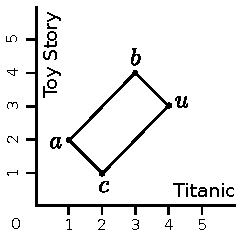
\includegraphics[width=2.5in]{figures/analogical_recommendation.pdf}
  \caption{Four users $a, b, c, u$ that are in proportion.}
\label{FIG:analogical_recommendation}
\end{figure}

\begin{table}[h!]
\centering
  \begin{tabular}{ c   c  c  c  c  c  }
\toprule
 & $j_1$ & $j_2$ & $j_3$ & $\cdots$ & $i$\\
  \midrule
$a$ & 1 & 4  & 3 & $\cdots$ & 2 \\
$b$ & 5 & 2  & 3 & $\cdots$ & 4 \\
$c$ & 1 & 5  & 3 & $\cdots$ & 3 \\
$u$ & 5 & 3  & 3 & $\cdots$ & ? \\
\bottomrule
\end{tabular}
\caption{The four users $a, b, c, u$ are in proportion for every item $j$ that
  they have commonly rated. For an item $i$ that $u$ has not rated, the
  prediction $\predrui$ is set as the solution of the analogical equation
  $2:4::3:?$, i.e. $\predrui = 3 - 2 + 4 = 5$, using the arithmetic proportion.}
\label{TAB:analogical_recommendation}
\end{table}

Just like with the conservative classifier, we will face the problem that in
practice, we may not find any $3$-tuple $a, b, c$ such that a perfect
proportion stands between $a, b, c$ and $u$. We will thus allow some distortion
of shape for the parallelogram $abcu$ by choosing another condition, for
example that $\norm{}{(a-b) - (c-u)} \leq \lambda$, where $\lambda$ is a
suitable threshold and $\norm{}{\cdot}$ is any $p$-norm. Note that this
relaxing of the definition of an analogical proportion exactly corresponds to
the usage of an analogical dissimilirity, so technically our algorithm is very
close to that of an extended classifier.

Our analogical proportion-based algorithm for recommendation is described by
Algorithm \ref{ALGO:analogical_recommendation}.
 \begin{algorithm}[!ht]
       \begin{algorithmic}

      \STATE {\bf Input}: A set of known ratings $R$, a user $u$, and an item
         $i$ such that $r_{ui} \notin R$.
      \STATE {\bf Output}: $\hat{r}_{ui}$, an estimation of $r_{ui}$.

      \STATE {\bf Init}:
      \STATE $C = \varnothing$ \quad \quad // The set of candidate ratings
      \FORALL{
        users $a, b, c$ in $U_i$ such that:\\
        \begin{itemize}
        \item $\norm{}{(a-b)-(c-d)}\leq \lambda$
        \item $r_{ai} : r_{bi} :: r_{ci} : y$ is solvable
        \end{itemize}
      }

      \STATE  $y \leftarrow r_{ci} - r_{ai} + r_{bi}$
      \STATE $C \gets C \cup \set{y}$ \quad // Add $y$ as a candidate rating
	  \ENDFOR

    \STATE $\hat{r}_{ui} = \aggr{y \in C} y$

\end{algorithmic}
     \caption{Analogical proportion-based algorithm for recommendation.}
       \label{ALGO:analogical_recommendation}
\end{algorithm}

We will note here an important point: while an extended classifier would look
for the $k$ $3$-tuples with the least values of analogical dissimilarity, we
here look for all three tuples whose AD is below some given threshold. This is
a common variant of the $k$-NN algorithm: you can either look for the $k$
nearest neighbors, or look for all instances that are within a given distance.

We have considered a strict condition for the solvability of the equation
$r_{ai} - r_{bi} = r_{ci} - y$: as the exact arithmetic result $y=r_{ci} +
r_{bi} -r_{ai}$ does not necessarily belong to the rating scale used in our
experiments (which is $[1,5]$), we have
considered that the equation is solvable only when $r_{ai}=r_{bi}$ or
$r_{ai}=r_{ci}$. In both cases, we ensure the solution $x \in
[1,5]$.\todo{tester avec juste appartenance}

Just like for the neighborhood approach described earlier, it is perfectly
possible to apply this algorithm in an in an item-based way rather
than in a user-based way. I.e. instead of looking for $3$-tuples of users, we
may look for $3$-tuples of items, etc. As both methods lead to similar result
with regard to the performances of the others recommendation algorithms, we
will only focus on the user-based approach described here.

In the next section, we will extensively study the performances of our
analogical recommender and compare it other standard recommendation algorithms.

\subsection{Experiments and results}
\label{results}

The performances of our analogical recommender are summed up in Table
\ref{TAB:parall_performances_comparison}. Various options were considered, that
we will describe in a moment. We also report the performances of other standard
recommendation algorithms that we have already mentioned:
\begin{itemize}
  \item The basic neighborhood approach (denoted $k$-NN) with different
    similarity metrics, namely Mean Squared Difference, Cosine similarity and
    Pearson similarity.  For these three algorithms, the size of the
    neighborhood was set to $k=40$
  \item The matrix-factorization algorithm (denoted MF), as described in section \ref{TODO}.
    The number of factors was set to $f = 100$, and the optimization problem
    was solved by a stochastic gradient descent of $20$ iterations with
    a constant learning rate of $0.005$ and a regularization penalty of $0.02$.
    These values are those recommended by the authors in \ref{TODO} for the
    Netflix dataset, and turned out to be quite efficient for our experiments.
  \item For the sake of completness we also report results for an algorithm
    that always predict the average of all ratings ($\predrui = \mu$ for all
    $u, i$), and for a random algorithm that predicts random ratings based on
    the distribution of the dataset, which is assumed to be normal.
\end{itemize}

The reported metrics are RMSE, precision, recall, F-measure, coverage, and
surprise. Precision, recall, F-measure and coverage  are reported as
percentages. Remember that for these dimensions high values mean high
performance, while for RMSE and surprise low values are better.  RMSE is the
only measure that only depends on the prediction algorithm $A$. All the other
dimension depend on the items that we actually choose to recommend, and as such
rely on the the recommendation strategy $S$. Here, we have chosen is to
recommend $i$ to $u$ if $\hat{r}_{ui} \geq 4$.

All reported results are averaged over a 5-folds cross-validation
procedure. Obviously, the five folds are the same for all of the algorithims,
to allow for meaningful comparisons.  The dataset that we used is the
Movielens-100K dataset\footnote{http://grouplens.org/datasets/movielens/},
composed of 100,000 ratings from 1000 users and 1700 movies. Each rating
belongs to the interval $[1, 5]$, and the sparsity of this dataset is of about
94\%, i.e. only 6\% of all possible ratings are actually known. We also
report the computation time of each algorithm (roughly estimated), which is not
an average but the total over the five folds.

\begin{table}[ht]
  \centering
\begin{tabular}{ l  l l  l  l  l  l   l  l  l  l }
\toprule
  Algorithm & \multicolumn{2}{ l }{Details}  & RMSE & Cov &  Prec & Rec & F & $\surpmax$ & $\surpavg$ & Time \\
\midrule
  \multirow{4}{*}{Parall} & \multirow{2}{*}{Sample}& $n=100$ & 1.18 &  57& 95 & 68 & 79
                          & .419& .166& 10m \\

                          & & $n=1000$ & 1.04 & 23 & 95 & 27 & 42
                          & .418 & .168 & 1h\\

                          & \multirow{2}{*}{$k$-NN}& $k=20$ & 1.00 & 31 & 97 & 38 & 54
                          & .421 & .176 & 6h\\

                          & & $k=30$ & 0.99 & 25 & 96 & 31 & 47
                          & .422 & .177  & 19h\\
\cmidrule(lr){1-3}
  \multirow{3}{*}{$k$-NN} & MSD& $k=40$ & 0.98 & 23 & 96 & 28 & 43 
                          & .423 & .175 & 30s\\
                          & Cos& $k= 40$& 1.02 & 21 & 96 & 26 & 41 &
                          .426 & .180 & 30s\\
                          & Pears& $k=40$ & 1.01 & 25 & 95 & 30 & 46 &
                          .425 & .170 & 30s\\
\cmidrule(){1-3}
                   MF & & $f = 100$ & 0.95 & 38 & 99 & 47 & 64 &  .422 & .178 & 45s\\
                   Mean &  & & 1.13 &  &  &  &  &   & & 1s\\
                   Random &  & &  1.52& 81 & 86 & 89 & 88 &  .432 & .155 & 1s\\
\bottomrule
\end{tabular}
\caption{Performances of recommendation algorithms on the Movielens-100k
  dataset.}
\label{TAB:parall_performances_comparison}
\end{table}

We have have considered various alternatives for our analogical
recommender. In fact, when trying to predict a single rating $\rui$, looking
for \textbf{all} the $3$-tuples of users in $U_i$ as described in Algorithm
\ref{ALGO:analogical_recommendation} is simply impractical\footnote{Remember
that $U_i$ is the set of user that have rated item $i$.}: there are often too
many users in $U_i$. As the complexity of this search is in $\mathcal{O}(\mid
U_i\mid^3)$ and as $\mid U_i\mid$ can be quite large for some items, strictly
sticking to Algorithm \ref{ALGO:analogical_recommendation} would lead to
even worse computation times. We thus have chosen two different strategies:
\begin{itemize}
  \item The first one is to randomly sample a $3$-tuple in $U_i^3$ $n$ times.
    As in the strict version of Algorithm \ref{ALGO:analogical_recommendation}
    the prediction is an average from all the $3$-tuples in $U_i^3$, choosing a
    large value of $n$ should lead to a fairly good estimate. We have reported
    the results for $n = 100$ and $n = 1000$. Note though that $\mid U_i
    \mid^3$ is usually much, much larger than 1000, so we only have very rough
    estimates here.
  \item The second one is to consider the $3$-tuples $(a, b, c)$ in the
    neighborhood of $u$, using the assumption that the neighbors of $u$ are
    probably more reliable to yield a prediction where $u$ is involved. We have
    used the MSD metric to compute neighborhood, and we have considered various
    sizes of neighborhood, namely $k = 20$  and $k = 30$. Unfortunately, values
    of $k$ greater than $30$ lead to basically never-ending algorithms.
\end{itemize}


\paragraph{Analysis\\}

Out of all the algorithm, the Matrix Factorization algorithm is by far the most
accurate, with and RMSE of 0.95. MF models were extremely popular during the
Netflix competition precisely because of their high accuracy. Note however that
even if the matrix factorization algorithms cannot be overlooked when it comes
to performance comparison, their philosophy remains quite different than that
of other classical neighborhood approaches. They tend to model data structures
at a high-level of abstraction, while neighborhood methods tend to model local
features of the data. As such, it makes more sense to compare the performances
of analogical recommenders to those of neighborhood-based techniques, rather
than use matrix factorization-based models as a baseline.

As expected, the RMSE of the
Parall Sample algorithm gets better while $n$ grows, but still
remains quite far from that of the $k$-NN algorithms. By paying attention to
the Parall $k$-NN algorithms, we see that looking for the
three-tuples in a the neighborhood of the users significantly improves the
accuracy of our analogy-based algorithms. Their RMSE is better than that of the
neighborhood approaches when using cosine and Pearson similarity, and it may
expected that using a neighborhood size of $k=40$ would lead the an RMSE close
to that of the $k$-NN algorithm with MSD similarity.

Let us now consider the coverage measure. At first sight, it may appear that
the Random and Parall Sample 100 algorithm have the best recall values. But this
would be missing a very important detail: any measure that evaluates the
fitness of the recommendation strategy $S$ (such as the coverage) greatly
depends \textbf{also} on the fitness of the prediction algorithm $A$, simply
because $S$ highly depends on $A$. Therefore, the coverage of the Random
algorithm cannot be taken very seriously, because its accuracy (RMSE) is
disastrous: it's only by chance that some items were estimated with a rating
greater than $4$, and then were recommended. The same goes for the Parall
Sample 100 algorithm, which has a quite bad accuracy.  Actually, the most
reasonable choice would probably the MF algorithm again, which has the best
RMSE and very decent coverage. With respect to coverage, our other
analogy-based algorithms yield comparable performances to the
neighborhood-based methods, with a slight advantage for analogy-based methods.

As for precision, recall and F-measure, we somehow have the same situation: the
Random algorithm seems to be the best one, but this need to be taken very
carefully. Here again, the MF algorithm seems to yield the best trade-off.
Comparatively, analogy-based algorithms have a slightly better F-measure than
the neighborhood approaches. This may describe the fact that our algorithms
tend to yield more diverse recommendations, as would also suggest the results
on the coverage.

The surprise measures are a bit more tricky to analyse. Looking at $\surpmax$,
which assess the least surprising recommendation (average over all users), we
see that the analogy-based algorithms tend to perform better, but the
$\surpavg$ measure counterbalances this observation. Undoubtely, the surprise
associated to a recommendation remains an extremely tricky concept to grasp and
to model, and the measures presented here only allow to assess a very rough
aspect.

As a side note, we have only reported the RMSE for the Mean algorithm, because
this algorithm always outputs a prediction of $\predrui = \mu = 3.53$ which is
lower than $4$, the threshold we chose for our recommendation strategy $S$.
Therefore, not a single item is recommended with this algorithm, and the
precision, recall, etc. are not defined (or simply 0).

We are now led to computation time... The nightmare of every analogical
proportion-based algorithm. All of the other algorithms can manage through the
five-folds cross-validation procedure in less than a minute, but our
analogy-based algorithms need hours to yield decent performances. This issue is
linked to the cubic complexity of the analogy-based learners, which cannot cope
with big amounts of data. For now, this limitation clearly prevents
analogy-based learners to be relevent in real-world applications such as
recommender systems.

\section{Clones}

Considering analogies between four users has shown to be computationally
intensive, thus not really suitable for recommendation purposes, where time is
a highly critical dimension. Yet, other forms of analogy can be addressed in
the recommendation task, based on the observation that some users may be more
inclined to give good (or bad) ratings than others. Indeed, ratings are in no
way absolute and greatly depend on the subjective appreciation each user has
about the rating scale. In the $[1, 5]$ scale for example, two users $u$ and
$v$ might semantically agree on an item $i$ describing it as $bad$, but there
is a chance that this agreement is not perfectly reflected in the ratings: $u$
might have rated $i$ with $r_{ui} = 1$ and $v$ with $r_{vi} = 3$, simply
because from $v$' point of view $3$ is a \textit{bad} rating, while for $u$ a
rating of $3$ would simply mean \textit{decent} or \textit{good enough}.  In
the following, we refer such users that \textit{semantically} agree on their
common items (but not necessarily \textit{numerically}) as \textit{clones}, as
illustrated in Figure \ref{FIG:alice_and_bob_clones}. Please note that the word
$clone$ is not used here to mean \textit{strictly identical}, but more in the
sense that two clones are two users following parallel paths.

\begin{figure}[!h]
\centering
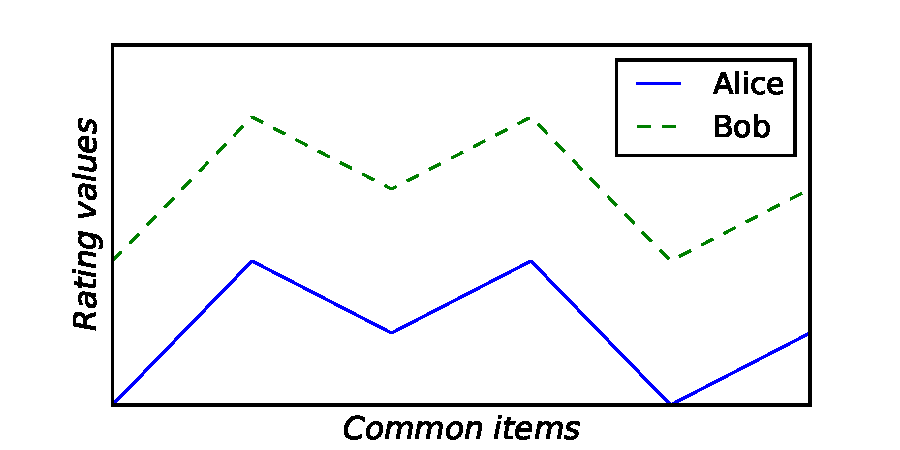
\includegraphics[width=4in]{figures/clones.pdf}
\caption{Bob is a perfect clone of Alice.}
\label{FIG:alice_and_bob_clones}
\end{figure}

It is obvious that in collaborative filtering, clones are of great interest
when it comes to predict a user's ratings, and yet the information they provide
is often discarded. Indeed, in Figure \ref{FIG:alice_and_bob_clones}, Alice and
Bob would definitly not be considered as neighbors, so Bob would not be used to
predict Alice's ratings, and Alice would not be used to predict Bob's ratings.
The principle underlying the analogical clone-based view is the following: for
predicting a missing rating for $u$, we not only look at its nearest neighbors
but also to those $v$ whose rating are such that $r_{ui} = r_{vi} + t_{vu}$
where $t_{vu}$ is a more or less constant \textbf{correction term} that can be
either positive or negative. This correction term is the difference between
Bob's ratings and those of Alice. When two users $u$ and $v$ are clones, we can
come back to an analogical proportion-based viewpoint by noticing that we have:
$$r_{ui} : r_{vi} :: r_{uj} : r_{vj},~~ r_{uj} : r_{vj} :: r_{uk} : r_{vk},
\dots,$$
where $i, j, k, \cdots$ are the common items of $u$ and $v$.


In the next two sections, we investigate this idea of a clone-based prediction,
first when ratings are viewed as numerical quantities in section
\ref{TODO}, and then when they have an ordinal meaning only in
section \ref{TODO}.

\subsection{Ratings as numerical quantities}

In the following, $C_i(u)$ will denote as the set of users that are clones of
$u$ and that have rated item $i$. From the previous unformal definitions, one
can easily derive a very general collaborative filtering framework for
predicting a user's rating by taking into account its clones: $$\predrui =
\aggr{v \in C_i(u)}(r_{vi} + t_{vu}),$$
where $t_{vu}$ is a \textit{correction term} that we need to add to $v$'s
ratings so that they correspond to those of $u$. We clearly have a
generalization of the neighborhood approach defined in Section \ref{TODO},
which we could write as:
$$\predrui = \aggr{\begin{subarray}{l}v \in C_i(u),\\ t_{vu} = 0\end{subarray}}(r_{vi} + t_{vu}).$$

Following this general framework, one can construct a great variety of
algorithms with various level of complexity. In the next subsections, we
propose a very straightforward algorithm, and a more efficient one.

\subsubsection{A straightforward prediction algorithm}
\label{STRAIGHTFORWARD}

We will first introduce the notion of $t$-clone. In its most simple form, a
user $v$ can be considered to be a $t$-clone of $u$ if the ratings of $v$
exactly differ from those of $u$ from a constant $t$:
$$
t\text{-}C(u) \eqdef \Set{v \in U | \forall i \in I_{uv},~ r_{ui} = r_{vi} + t}.
$$
From then on, computing $\predrui$ amounts to finding all the users $v$ that
satisfy this criteria, and computing an aggregation of their rating for $i$,
which can simply be an average. We implemented this basic algorithm described
by algorithm \ref{ALGO:bruteforce}, and referred to as \textit{brute-force}.

 \begin{algorithm}[!ht]
   \caption{A brute-force algorithm for clone-based recommendation.}
       \label{ALGO:bruteforce}
       \begin{algorithmic}

      \STATE {\bf Input}: A set of known ratings $R$, a user $u$, an item
      $i$ such that $r_{ui} \notin R$.
      \STATE {\bf Output}: $\hat{r}_{ui}$, an estimation of $r_{ui}$

      \STATE {\bf Init}:
      \STATE $C = \varnothing$ \quad \quad // list of candidate ratings
      \FORALL{ users $v \in U_i$}
        \FORALL{$t$}
          \IF{$v \in t\text{-Clones}(u)$}
          \STATE $C \gets C \cup \{r_{vi} + t\}$ \quad // add x as a candidate rating
          \ENDIF
        \ENDFOR
	    \ENDFOR
    \STATE $\hat{r}_{ui} = \aggr{c \in C} c$
\end{algorithmic}
\end{algorithm}

Of course, one may want to relax the definition of a $t$-clone, as the current
one is too strict and only very few users will satisfy this criteria. In our
implementation, we chose the following condition:
$$
t\text{-}C(u) \eqdef \Set{v \in U |  \sum_{i \in I_{uv}} |(r_{ui} - r_{vi}) -
t| \leq \mid I_{uv}\mid},$$
which amounts to accept $v$ as a $t$-clone of $u$ if on average, the
difference $|r_{ui} - r_{vi}|$ is equal to $t$ with a margin of $1$.
The values of $t$ clearly depend on the rating scale. The datasets on which we
tested our algorithms use the $[1, 5]$ interval, so possible values for $t$
that were have considered are integer values in $[-4, 4]$.

This is obviously a very rough algorithm, to which one could point out numerous
flaws. The first obvious one is its time complexity which is very high, but the
purpose of this brute-force algorithm is simply to show that even such a basic
clone-based approach can lead to better results than a basic neighborhood
method, as we will see later.

\subsubsection{Modeling clones with the similarity measure}
Another option to consider clones is to use the well known neighborhood-based
formula, and capture their effect inside an appropriate similarity measure.
Recall that the general neighborhood formula is as follows:

$$\predrui = \frac{\sum\limits_{v \in N_i^k(u)} r_{vi} \cdot \ssim(u, v)}
{\sum\limits_{v \in N_i^k(u)}\ssim(u, v)}.$$

We have seen that this formula is commonly used with classical similarity
metrics such as Pearson similarity, cosine similarity, or inverse of MSD.
However, these similarities are not plainly satisfactory when it comes to
clones. Indeed with these metrics, two users are considered to be close if
their common ratings are often the same, but two perfect clones $u$ and $v$
with a significant correction term $t_{vu}$ would be considered as far from
each other, thus involving a loss of information.

We propose the following simple choice of metric to measure how two users
relate as clones:
$$\clonedist(u, v) \eqdef  \frac{1}{\mid I_{uv} \mid} \cdot
\sum\limits_{i \in I_{uv}} \left[(r_{ui} - r_{vi}) - \mu_{uv}\right]^2$$
where $\mu_{vu}$ is the mean difference between ratings of $u$ and $v$:
$$\mu_{uv} \eqdef \frac{1}{\mid I_{uv}\mid}\sum_{i \in I_{uv}} (r_{ui} -
r_{vi}).$$

We can understand this distance in two ways:
\begin{itemize}
\item it can be regarded as the variance of the difference of ratings between
  $u$ and $v$,
\item or it can be regarded as a simple MSD measure (defined in Section
  \ref{TODO} to which the mean difference of ratings between $u$ and $v$ has
    been subtracted.
  \end{itemize}

As our measure $\clonedist$ is a distance, it is necessary to transform it into
a similarity measure. Common choice is to take its inverse (while accounting
for zero division):
$$\clonesim(u, v) = \frac{1}{\clonedist(u, v) + 1}.$$

\noindent
Once we know how to find the clones of a user, it is a simple matter to output
a prediction using the classical neighborhood approach:
$$\predrui = \frac{\sum_{v \in N_i^k(u)} (r_{vi} + \mu_{uv}) \cdot \clonesim(u,
v)}{\sum_{v \in N_i^k(u)} \clonesim(u, v)}.$$

This algorithm will be referred to as Clone. For the sake of completeness, we
also tried the same formula but with a more basic similarity metric that does
not care about clones: MSD.

\subsubsection{Current advances in neighborhood-based techniques}

What we have seen so far in terms of neighborhood methods are the rough, basic
techniques that have existed for a long time. Actually, more sophisticated
approaches have been developed, in particular during the Netflix competition.
The one we will describe here has been popularized in \cite{BelKorSIGKDD2007},
and makes use of \textbf{baseline predictors}:
$$\predrui = b_{ui} + \frac{\sum\limits_{v \in N_i^k(u)} (r_{vi} - b_{vi})
\cdot \ssim(u, v)} {\sum\limits_{v \in N_i^k(u)}\ssim(u, v)}.$$
where $b_{ui}$ is a baseline (or bias) related to user $u$ and item $i$. Its
expression is $b_{ui} = \mu + b_u + b_i$, where $b_u$ is supposed to model how
$u$ tends to give higher (or lower) ratings than the average of all ratings
$\mu$, and $b_i$ is supposed to model how $i$ tends to be rated higher or lower
than $\mu$. For example, if the mean of all rating is $\mu = 3$, and the
ratings of a user are $(2, 2, 1)$, its bias $b_u$ would be close to $-1$.

Baselines are computed by solving a regularized least squares problem:
$$\min_{b_u, b_i} \sum_{r_{ui} \in R} \left[r_{ui} - (\mu + b_u + b_i)\right]^2
+ \lambda \left(b_u^2 + b_i^2 \right).$$
which can be achieved efficiently by stochastic gradient descent, or
alternating least squares. The regularization terms are here to avoid
overfitting: they allow to give more confidence to biases that are computed on
a high number of ratings. In our previous example, the user had only rated $3$
items so we cannot say reliably say that its real bias is really close $-1$.
This regularization can actually be justified using a Bayesian view, but we
will not describe it here.

In their work, the author have used this particular similarity metric, that is
in perfect accordance with their prediction formula:
$$\text{sim}(u, v) = \frac
{ \sum\limits_{i \in I_{uv}} (r_{ui} -  b_{ui}) \cdot (r_{vi} - b_{vi})}
{\sqrt{\sum\limits_{i \in I_{uv}} (r_{ui} -  b_{ui})^2} \cdot
\sqrt{\sum\limits_{i \in I_{uv}} (r_{vi} -  b_{vi})^2}}.$$

It is simply a Pearson correlation coefficient, except that instead of
centering ratings by their means, they are centered with the baseline
predictors. This simingly simple tweaks actaually has various consequences that
are very interesting. An intuitive and illuminating way to look at this
algorithm as a whole is to see that it conceptually follows these steps:
\begin{enumerate}
  \item Compute $R'$, the set of all ratings normalized by the corresponding
    baselines: $r'_{ui} = r_{ui} - b_{ui}$.  $R'$ can be regarded as the set
    where all ratings are given from the same frame of reference, thus
    discarding any bias coming from the users or from the items. In $R'$
    ratings can then be considered as absolute, in the sens that they are not
    spoiled by the users moods or the items inherent popularity.
  \item Using $R'$, compute similarities between users using the cosine
    similarity (the cosine similarity is the same as the Pearson correlation
    coefficient, except that quantities are not centered).
  \item Output a prediction using the basic neighborhood formula. As this
    prediction belongs to the same space of $R'$ where ratings have no bias, it
    needs to be transposed back to the space of $R$ for performance evaluation
    purposes. This is why $b_{ui}$ and $b_{vi}$ are added (or subtracted) in
    the prediction formula of $\predrui$.
\end{enumerate}
\noindent
In what follows, this algorithm will be referred to as $\knns$.

It is very clear that the use of the baseline predictors and the use of
clone-based recommendation are motivated by the same reasons: they both come
from the fact that users (and items) tend to interpret differently the rating
scale.  This means that $\knns$ implicitly takes the idea of clones into
account, and thus a form of analogical reasoning.  Differences and resemblances
of these two approaches will be discussed in the next section.

\subsubsection{Experiments and discussion}
\label{expeDiscuss}

To assess the suitability of our clone-based view of recommendation, we have
evaluated the accuracy of the brute-force and Clone algorithms, and compared
them to the previously mentioned approaches: the basic neighborhood method, and
the neighborhood method taking into account user and item biases. The
evaluation protocol is the same as that of Section \ref{TODO}, i.e. results are
averaged over a 5-folds cross-validation procedure. In addition to
the Movielens-100k dataset presenter earlier, we also used the Movielens-1M
dataset containing 1 million ratings with 6000 users and 4000 movies.
For each of these algorithms, the number of neighbors or clones used to output
a prediction is $k = 40$, except for the brute-force algorithm where the number
of clones can not be controlled. The RMSE and MAE of the algorithms are
reported on Table
\ref{TAB:clone_based_rmse_mae}.

\begin{table}[ht]
  \centering
  \begin{tabular}{ l  l  l  l  l l l }
\toprule
    & & &  \multicolumn{2}{ c }{ML-100k}  & \multicolumn{2}{ c }{ML-1M} \\
  \cmidrule(lr){4-5}
  \cmidrule(lr){6-7}
    Algorithm& Details  & & RMSE & MAE  & RMSE & MAE \\
\midrule
    $k$-NN & MSD & $k=40$&  .979 & .773 & .921 & .725\\
    Brute-Force &  & & .948 & .737 & & \\
  \cmidrule(lr){1-2}
    \multirow{2}{*}{Clone} & \clonesim & $k=40$& .936 & .733 & .899& .705\\
                           & MSD & $k=40$ &  .931 &  .732 & .897 &  .707\\
  \cmidrule(lr){1-2}
    $\knns$ & & $k=40$ & .921 & .721 & .869& .680\\
\bottomrule
\end{tabular}
  \caption{RMSE and MAE of our clone-based algorithms on the movielens 100k and
  1M datasets.}
  \label{TAB:clone_based_rmse_mae}
\end{table}

It is very clear that even a very straightforward approach of the clone-based
recommendation principle significantly outperforms the most basic $k$-NN
algorithm, and thus validates the need to take into account biases between
users. The brute-force is however a lot heavier to compute, and thus not very
suitable for real world recommendation purposes (its performances on the
Movielens-1M dataset simply could not be computed). The two other clone-based
algorithms however, have the exact same complexity of any $k$-NN-based
algorithm which is a significant improvement from the algorithm described in
section \ref{TODO}.

Our two Clone algorithm output (almost) exactly the same
accuracies. This may seem a bit surprising, because the Clone MSD algorithm
does not take into account clones in the similarity measure, and we would
expect it to yield a lower accuracy. But this result still gives a further
reason to consider clones as useful predictors: the only difference between the
Clone MSD algorithm and the $k$-NN MSD algorithm (whose accuracy is much worse)
is that in the prediction of Clone MSD, the mean differences $\mu_{uv}$ between
the ratings of $u$ and its neighbors are taken into account.

Performances of the Clone algorithms are close to those of the state of the
art $\knns$ algorithm, yet the difference is more striking on the Movielens-1M
dataset. It is however important to understand that these
algorithms differ on the following points:
\begin{itemize}
\item The Clone algorithms do not address item bias, which is a significant
  drawback. It may not be unreasonable to believe that incorporating item bias
  in the prediction would lead to better results.
\item There is a subtle yet meaningful difference of interpretation between the
  biases induced by both algorithms. In the Clone algorithm, biases are all
  pairwise, meaning that they involve two users, and they are computed on items
  that both users have rated. As for the $\knns$ algorithm, there is no such
  thing as a pairwise bias. Bias for a given user is computed using only its
  own ratings, and is a result of a global optimization problem involving the
  global mean of all ratings, which means that every single rating in $R$ has
  an impact on the bias.
\item On the biggest dataset (Movielens-1M), the $\knns$ algorithm appears to
  achieve better accuracy than the other algorithms, while this is not the case
  for the small dataset. A possible explanation is that as baselines are
  computed on the whole training set, they tend to capture most of the noise
  when the training set gets bigger, thus improving accuracy compared to more
  heuristic-based approach.
\end{itemize}

It should also be noted that in practice, it is recommended to perform a
shrinkage on the similarity measure of algorithm $\knns$, in order to take into
account the number of common items between two users: the more items they
share, the more confident we are when computing their similarity
\cite{KorACM2010}. Such techniques can further improve both RMSE and MAE of the
algorithm.  Similarly, in the clone-based approach, it might be of interest to
discount clones that rely on a too small number of common items.

\subsection{Towards an ordinal view of ratings}
\label{ORDINAL_POV}

We may wonder if one can devise a counterpart of the numerical clone-based
approach, which would be compatible with an ordinal view of the ratings.
Indeed, an extreme way for unbiasing and comparing two sets of ratings is to
forget about their numerical values, and only consider their rankings.  The
idea of viewing ratings in a ordinal manner has been advocated in
\cite{KorSillRECSYS11}.
In this section, we discuss an ordinal counterpart of the analogical approach
previously presented.  Analogical reasoning with ordinal data has first been
proposed in \cite{MicBarCAP09}, yet with a different concern.

\subsubsection{An algorithm for rank prediction}
Indeed the idea that ``\textit{the rating of user $u$ for item $i$ is to the
rating of user $v$ for item $i$ as the rating of user $u$ for item $j$ is to
the rating of user $v$ for item $j$}’’ may be understood  as well in an ordinal
manner. This leads to state that ``\textit{the relative ranking of item $i$
  among the ratings given by user $u$  is to the relative ranking of item $i$
  among the ratings given by user $v$ as the relative ranking of item $j$ among
  the ratings given by user $u$  is to the relative ranking of item $j$ among
the ratings given by user $v$}.

This means that we need to compare the rankings given by two users $u$ and $v$
on their common items. In the following, $\rho_{ui}$ denotes the relative
ranking of item $i$ out of all the items rated by $u$. Our goal is to estimate
all values of $\rho_{ui}$, for any user and any item. The main steps of a
possible algorithm is as follows:
\begin{enumerate}
  \item Compute similarities between users, based on their rankings. A very
    popular similarity ranking measure is the Spearman's rank correlation
    coefficient, or Spearman's rho.
  \item Compute an estimated rank $\hat{\rho}_{ui}$ as an aggregation of all the
    rankings $\rho_{vi}$ extracted from the $k$ nearest neighbors (using
    Spearman's rho as similarity):
    $$\hat{\rho}_{ui} = \frac{\sum_{v \in N_i^k(u)} \rho_{vi} \cdot
    sim(u, v)}{\sum_{v \in N_i^k(u)} sim(u, v)}.$$
\end{enumerate}

This is obviously very similar to the neighborhood approach described in
section \ref{MODELING_CLONES}, but instead of predicting a rating, we output a
predicted rank. This approach is denoted as \textit{RankAnlg}.


\subsubsection{Experiments}

We evaluated the performance of our algorithm and compared it to other
previously described approaches, using the exact same evaluation protocol as in
section \ref{expeDiscuss}. The Movielens-1m dataset was not benchmarked, as our
algorithm is too computationally intensive.

RMSE and MAE are good measure for evaluation rating prediction accuracy, but
are not suitable when it comes to evaluate rankings. A better measure is the
Fraction of Concordant Pair, which evaluates the probability that given any two
items $i$ and $j$ rated by any user $u$, the system has correctly estimated
whether $u$ prefers $i$ over $j$ or the inverse. To compute the FCP, we need to
intermediate measures. $c_u$ defines the number of concordant pairs for user
$u$, and $d_u$ its number of discordant pairs. The FCP is then computed over all
users as the proportion of concordant pairs.

\begin{align*}
  c_u &\eqdef \Set{(i, j) \in I^2 \quad | \quad \predrui > \predruj \text{ and
  } r_{ui} > r_{uj}},\\
  d_u &\eqdef \Set{(i, j) \in I^2 \quad | \quad \predrui \geq \predruj \text{
    and } r_{ui} < r_{uj}},\\
  \FCP &\eqdef \frac{\sum\limits_{u \in U} c_u}{\sum\limits_{u \in U} c_u +
  \sum\limits_{u \in U} d_u}.
\end{align*}
Note that $\predrui$ here may represent either a rating prediction or a
ranking prediction $\hat{\rho_{ui}}$.

Results are reported in table \ref{table:res100kRank}.

\begin{table}[!ht]
\centering
\begin{tabular}{ l l  l l }
\toprule
     & RankAnlg &  k-NN & $\knns$\\
\midrule
\FCP  &  .7063   & .7096 &  .7163   \\
\bottomrule
\end{tabular}
\caption{\FCP of our rank prediction algorithm on the Movielens-100k
  dataset.}
\label{table:res100kRank}
\end{table}

Unfortunately, even a basic algorithm that was not designed for ranking
prediction performs better in terms of FCP. To explain this difference, one may
look at the distribution of average support over all the predictions, as shown
on figure \ref{FIG_SUPPORT}. Between
two users $u$ and $v$, the support is defined as the number of common items
($|I_{uv}|$), which was used to compute the similarity between $u$ and $v$. For
a given prediction $\predrui$, the average support is the average of all the
supports $|I_{uv}|$ over all users $v \in N_i^k(u)$.

\begin{figure}[!h]
\centering
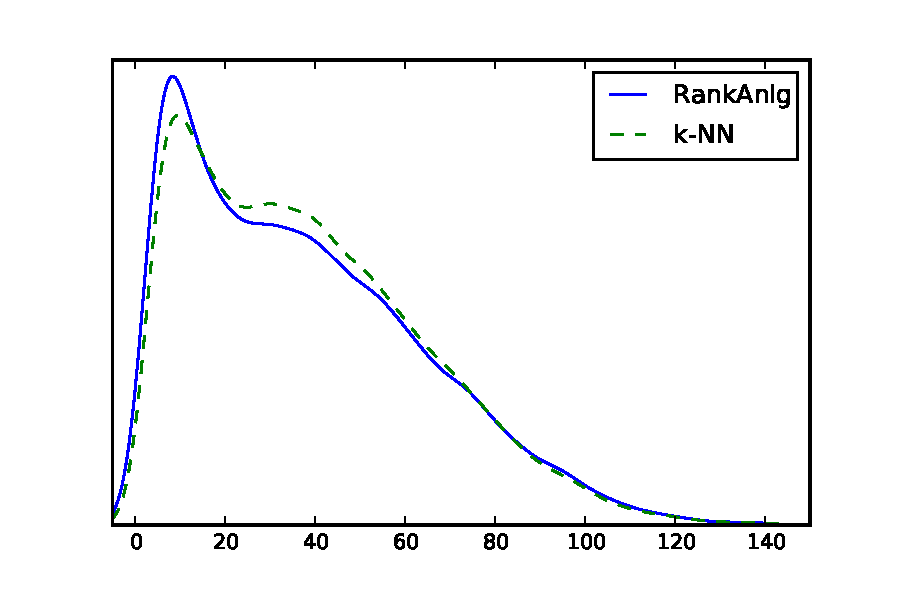
\includegraphics[width=2.5in]{figures/support.pdf}
\caption{Distribution of average support.}
\label{FIG_SUPPORT}
\end{figure}

The use Spearman's rho tends to provide with neighbors that have smaller
support, thus leading to a less significant and less accurate estimation of the
neighborhood, which may explain the differences in performance.

\section{Mining analogical proportions}

\subsection{Association rules}

Association rules are pieces of information that one can extract from a
database, and that reveal dependencies between items. Recommendation is one of
the principal application of association rules. Strating from the association
rule $i \implies j$, which means that users that buy $i$ tend to buy $j$ with
high probability, a recommendation system can suggest $j$ as soon as we bought
$i$ but not yet $j$. A concrete example of association rule We will here
formally defined association rules.

Let $I = \Set{i_1, i_2, ..., i_m}$ be a set of items, and let $T = \Set{t_1,
t_2, ..., t_n}$ be a multiset of transactions, where each transaction is a
subset of $I$: $t_i \subseteq I$. A transaction simply is a set of items that
are bought together. An association rule is expressed in the form $ X \implies
Y$, where $ X \subset I, ~ Y \subset I$, and $X \cap Y = \varnothing$. $X$ and
$ Y $ are sets of items (also called \textbf {itemsets}), and the
\textbf{support} $\supp (X) $ of an itemset $X$ is defined as the proportion of
transactions that contain it:
$$\supp(X) \eqdef \frac{\mid \Set{t \in T | X \subseteq t}\mid}{\mid T \mid}.$$
A number of measures can be used to evaluate the quality of an
association rule, such as the \textbf{trust} which can be expressed as:
$$\text{Trust}(X \implies Y) \eqdef \frac{\supp (X \cup Y)}{\supp (X)}.$$
As could be naturally expected, $\text{Trust}(X \implies Y)$ is equal to $1$
when the items of $X$ and $Y$ are systematically bought together and decreases
if the set $X$ is sometimes found in a transaction that does not contain $Y$.

The mining of association rules is a popular research topic, and has been
extensively studied. The most famous algorithm for association rule mining
probably is the \textbf{Apriori} algorithm, introduced in \cite{AgrSriVLDB94}.
This algorithm relies on the simple (but strong) fact that if an itemset $X$ is
of size $s$, then any of the subsets

Les méthodes d'extraction de telles règles ont fait l'objet de nombreuses
études. L'algorithme {\it Apriori} \cite{AgrSriVLDB94} est probablement le plus
connu mais il en existe d'autres.  L'idée   est de fixer un seuil minimum
$\alpha$ pour le support et de chercher dans $2^I$ les itemsets dont le support
dépasse $\alpha$, pour obtenir un ensemble $S$ d'itemsets fréquents. Cette
recherche est facilitée par le fait que tout sous-ensemble d'un itemset
fréquent est aussi fréquent.

On se fixe alors un nouveau seuil $\beta$ pour la confiance.  Dès lors que
l'on dispose d'un itemset $IS$ de $S$, on peut chercher toutes les partitions
de $IS$ sous la forme $X \cup Y = IS$, calculer la confiance de la règle $X
\rightarrow Y$, ne garder cette règle que si sa confiance dépasse le seuil
$\beta$.

L'algorithme retourne finalement un ensemble de règles d'association
respectant les critères de qualité exigés, et fournissant donc un certain
nombre d'informations sur les liens entre les éléments de la base de
données.
%Sur le mode des proportions analogiques, on admettra que {\it le dentifrice
%est à la brosse à dent ce que le beurre est à la biscotte}.  Dans ce
%cas, on peut penser recommander à quelqu'un ayant acheté dentifrice,
%brosse à dent et beurre, d'acheter des biscottes. Sur quelle base?  Sur la
%base que la relation liant dentifrice et brosse à dent est la même que
%celle liant beurre et biscottes.
Au même titre que les règles d'association, la détection de proportions
analogiques dans une base de données est une information supplémentaire
fournie aux détenteurs de la base.  Dans la section suivante, nous
utilisons l'algorithme {\it Apriori} pour extraire d'une base des proportions
analogiques.

\subsection{Trouver des analogies}
Dans la suite, on recherche des analogies dans une base de données dédiée à la
recommandation.
L'objectif d'un système de recommandation est de fournir à un utilisateur une
liste personnalisée d'articles susceptibles de l'intéresser.  Soit $U$ un
ensemble d'utilisateurs et $I$ un ensemble d'items. Pour certaines paires $(u,
i) \in U \times I$, on connait la note $r_{ui}$, qui exprime l'intérêt que
l'utilisateur $u$ porte à l'item $i$ : on trouvera souvent $r_{ui} \in
[\text{aime, n'aime pas}]$ ou bien $r_{ui} \in [1, 2, 3, 4, 5]$. Nous dénotons l'ensemble des notes
connues du système par $R$.
% Pour recommander des articles aux utilisateurs, un
%système de recommandation procède ainsi: i) avec un algorithme $A$, on estime
%les notes $r_{ui}$ inconnues (c.à.d.  $r_{ui} \notin R$);
%Cette estimation  $A(u, i)$ est communément notée $\hat{r}_{ui}$.
%ii) Avec une stratégie de recommandation $S$ et au vu des notes précédemment
%estimées, recommander des items aux utilisateurs.
%Par exemple, une stratégie très basique mais assez courante est de suggérer à
%$u$ les articles $i$ pour lesquels $\hat{r}_{ui}$ est le plus grand.


Notre approche s'applique donc au cas o\`u peu de notes sont connues.  Considérons
4 items  $A, B, C$ et $D$ pour lesquels on cherche à savoir s'ils constituent
une analogie valide, sans avoir pour l'instant d'idée sur l'ordre dans lequel
on doit les considérer. Comme pour les règles d'association, la notion de
support demeure puisque ces 4 items constituent un 4-itemset.  Par
définition:

%\small
$Supp(\{A, B, C, D \})= \frac{|U_{ABCD}|}{|U|}$, où $U_{ABCD}$ est l'ensemble
des utilisateurs qui ont conjointement noté $A, B, C,$ et $D$.

%Dans le cas d'une base de données de films comme MovieLens, le support de 4
%films $\{a, b, c, d \}$ est simplement la proportion d'utilisateurs ayant vu
%ces 4 films.
Naturellement, comme pour les règles d'association, on peut ne
s'intéresser qu'aux analogies dont le support est supérieur à un certain
seuil $\alpha$.  Ensuite, pour un itemset $\{A, B, C, D \}$ de support
supérieur au seuil $\alpha$ que l'on s'est fixé, et ayant à notre
disposition une relation analogique permettant d'affirmer si, par exemple,
$A:B::C:D$ est valide ou non, on cherche quelles sont les analogies possibles.

On sait qu'il y a 4! = 24 permutations possibles de $\{A, B, C, D \}$,
correspondant à 24 analogies possibles. Cependant, compte tenu des
propriétés de l'analogie, un certain nombre d'entre elles sont
équivalentes et mènent à 3 classes de 8 analogies équivalentes
représentées par:
\begin{itemize}
\item $A:B::C:D$
\item $A:B::D:C$
\item $A:D::C:B$
\end{itemize}
Il convient donc de ne chercher que ces trois classes d'analogies.  Pour ce
faire, on pourra se donner une fonction $f$ évaluant la qualité d'une
analogie, un autre seuil de qualité $\beta$, et ne retenir, parmi les trois
options possibles que celles dont la qualité dépasse le seuil $\beta$. Ce que
nous appelons la qualité ici joue le rôle de la confiance pour les règles
d'association.  En clair $A:B::C:D$ est retenue comme analogie  valide si et
seulement si $f(A:B::C:D) \geq \beta$.  A la fin de cette procédure, on obtient
donc un ensemble d'analogies qui représentent des relations entre quatre items.

\subsubsection{Exemples de fonction de qualité}
Tous les 4-itemsets considérés $A, B, C, D$ sont représentés par
des vecteur de notes.  La dimension de ces vecteurs est égale au nombre
d'utilisateurs ayant noté les quatre items.  Cela nous donne plusieurs options
pour mesurer la qualité d'une proportion $A:B::C:D$, qui dépend de la nature
des analogies considérées et donc implicitement de l'échelle de notes.

Dans le cas d'une échelle binaire ($r_{ui} \in [\text{aime, n'aime pas}]$), on
pourra choisir pour $f$ la proportion de composantes pour lesquelles l'analogie
tient parfaitement.  Si l'échelle est numérique, on dispose de plusieurs
techniques pour évaluer l'exactitude d'une proportion entre quatre réels, qui
donneront des valeurs entre 0 et 1. Là aussi, on peut envisager une
aggrégation de ces valeurs de vérité.  Toujours si l'échelle est réelle et en
utilisant la proportion arithmétique, on sait que $A, B, C, D$ forment un
parallèlogramme ssi l'analogie est parfaite. La qualité d'une analogie
$A:B::C:D$ est donc inversement proportionnelle à la déformation du
parallélogramme dans $\mathbb{R}^n$, que l'on peut calculer en termes de
distance euclidienne.  Enfin, en adoptant un point de vue statistique on peut aussi
s'intéresser à la probabilité d'observer $A:B::C:D$, et considérer que la
proportion est crédible si elle a peu de chance d'être dûe au hasard (voir
Section \ref{expe}).

\subsubsection{Algorithme}
L'algorithme d'extraction de règles analogiques est alors calqué sur le modèle
d'extraction de règles d'association : on se donne une fonction de qualité $f$,
et deux seuils $\alpha$ et $\beta$.

D'abord, on calcule tous les 4-itemsets de support supérieur au seuil $\alpha$
à   l'aide de l'algorithme \textit{Apriori}.  Pour chaque itemset retenu,
on calcule la qualité des trois formes possibles non équivalentes d'analogie, et on garde celles dont
la qualité dépasse le seuil $\beta$.

\begin{enumerate}
\item Entrée: une relation d'analogie, une fonction de qualité $f$, deux seuils
  $\alpha$ et $\beta$.
\item Calculer tous les 4-itemsets de support supérieur au seuil $\alpha$ à
  l'aide l'algorithm \textit{Apriori}.
\item Pour chaque itemset retenu, calculer, parmi les 3 formes possibles non
  équivalentes d'analogie, celles dont la qualité dépasse le seuil $\beta$.
\item Sortie : la liste des règles analogiques retenues.
\end{enumerate}

\subsection{Premières expériences}

Nous avons expérimenté cet algorithme sur la base de données
Movielens\footnote{http://grouplens.org/datasets/movielens/},
constituée de $100~000$ notes de $1700$ films par $1000$ utilisateurs. Chaque
note appartient à l'échelle $[1, 2, 3, 4, 5]$, mais nous l'avons ramenée à une
échelle binaire de la façon suivante : un utilisateur $u$ aime un film s'il lui
a attribué une note supérieure à $\mu_u$, où $\mu_u$ est la note moyenne que
$u$ donne aux films qu'il a vus.

En plus de choisir un critère de support minimal, nous avons aussi imposé un
support maximal : les films très populaires vus par beaucoup de monde font
généralement consensus (les gens les apprécient), et ont peu de chance de
construire des analogies intéressantes. Cela a de plus l'avantage de réduire
l'espace de recherche, et donc accélerer significativement la recherche de
4-itemsets. De plus, toujours dans le but d'éviter de construire des analogies
trop triviales, on ne retient pas les proportions de la forme $x:x::x:x$.

En choisissant un support minimal de 40 et un support maximal de 150, nous
obtenons les mesures de qualités (calculées comme la proportion d'analogies
parfaites) illustrées par la figure \ref{qualite}. Comme on peut le voir, la
meilleure proportion a une qualité d'environ $40$\%, ce qui peut paraître peu
convainquant. Néanmoins, en remarquant que pour une composante il y a 4 chances
sur 16 d'obtenir une analogie significative (on ignore les $x:x::x:x$), et en supposant que les composantes sont
indépendantes les unes des autres, le nombre de composantes pour lesquelles
l'analogie est vraie suit une loi binomiale de paramètres $\mathcal{B}(40,
\frac{1}{4})$, où $40$ est la dimension des vecteurs. Sous ces hypothèses, la
probabilité d'obtenir $40$\% ou plus d'analogies parfaites est de $0.026$, ce qui
tend à montrer qu'un tel quadruplet d'items reste significatif, en cela que la
proportion analogique observée a peu de chance d'être due au hasard.

\begin{figure}[h]
  \vspace{-0.4cm}
\caption{Qualité des proportions trouvées}
\label{qualite}
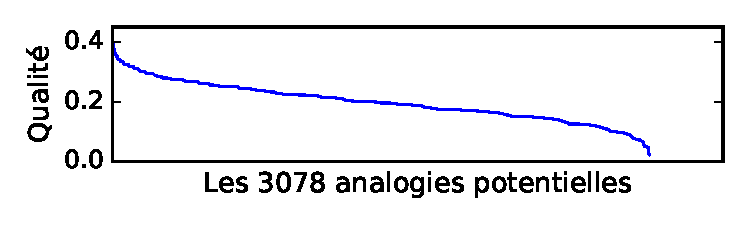
\includegraphics[scale=0.6]{figures/quality_of_proportions.pdf}
\vspace{-0.4cm}
\end{figure}
Les mêmes expériences ont été menées en gardant l'échelle de notes numérique
($[1, 2, 3, 4, 5]$) et en utilisant une expression multivaluée de l'analogie.
Les meilleures proportions obtenues s'avèrent être globalement les mêmes que
celles qui ressortent de l'échelle binaire, montrant ainsi la cohérence des
deux approches. La m\'ediocre qualit\'e des proportions analogiques trouv\'ees,
m\^eme si elles sont statistiquement significatives,
ne permet pas d'utiliser raisonnablement l'inf\'erence analogique dans cet exemple.
Ceci  tend \`a expliquer a posteriori pourquoi une approche pour la
pr\'ediction de notes manquantes, bas\'ee sur la recherche de triplets
analogiques, avait obtenu des r\'esultats modestes \cite{HugPraRicISMIS15}.
